\section{Transformers: More Than Meets the Eye}
\label{lab_transformers}

%\makelabheader %(Space for student name, etc., defined in master.tex)

\bigskip

\begin{enumerate}[wide]

\item Your transformer, shown in the circuit diagram below, has two primary coils and two secondary coils that can be wired in a variety of ways to yield different effective turn ratios $N_1/N_2$.  Wire the circuit as shown below, using your oscilloscope to measure the RMS voltages $V_1$ and $V_2$.  (Note: the wires may come out of your transformer in a different order than is shown here; ignore the order and go by the colors.)  Based on your measurements, what is the apparent turns ratio of the transformer as it is connected here?  Is this a ``step down'' or ``step up'' transformer?  

\begin{center}

\includegraphics{transformers/transformer_par_single.eps}
\end{center}

\item Predict the value of the secondary voltage $V_2$ if the transformer wiring is changed as shown below, with the two secondary coils now connected in parallel, just as the two primary coils are.  Test your prediction.

\begin{center}
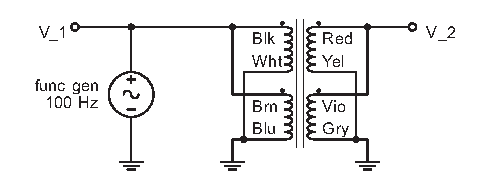
\includegraphics{transformers/transformer_par_par.eps}
\end{center}

\item If you look closely at the transformer wiring diagrams above, you'll see that some of the transformer terminals have a small dot near them.  This denotes an arbitrary polarity of the coils.  Essentially, although it doesn't matter whether the two secondary coils are wound around clockwise or counterclockwise, it \textit{does} matter that both are wired the same direction.  Predict what will happen if you reverse the polarity of one of the coils as shown below, and test your prediction with a measurement.

\begin{center}

\includegraphics{transformers/transformer_par_par_reversed.eps}
\end{center}

\item Predict what secondary voltage $V_2$ you will measure if your circuit is rewired so that the two primary coils remain in parallel, but the two secondary coils are connected in series, as shown below.  Test your prediction with a measurement.  What is the turns ratio for the transformer when it is wired this way?

\begin{center}
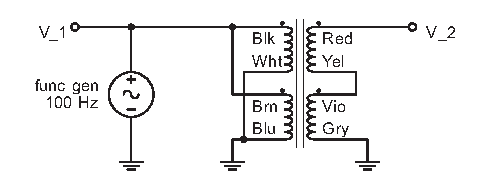
\includegraphics{transformers/transformer_par_ser.eps}
\end{center}

\item Predict the secondary voltage $V_2$ and the turns ratio of the transformer if the circuit is rewired so that both the primary coils and the secondary coils connected in series. Test your prediction with a measurement.  (You may find that the primary voltage has also changed slightly from the previous part, due to the internal resistance of the function generator.)

\item In the circuit shown below, both pairs of coils are still connected in series as before, but the roles of the primary and secondary have now been reversed.  Measure the voltages $V_1$ and $V_2$.  In this new configuration, is this a ``step down'' or ``step up'' transformer?  What is the turns ratio?  Is this consistent with your measurement in the previous part? 

\begin{center}

\includegraphics{transformers/transformer_ser_ser_inverted.eps}
\end{center}

\item What accounts for the slight descrepancy between the apparent turns ratios you measured in the last two parts?


\end{enumerate}

\textit{If a transformer steps the voltage UP, it has to step the current DOWN and vice-versa.  (If it stepped both of them up, then it would be stepping up the power.  If it could do that, then our nation's energy problems would be solved.)  The way the transformer ``steps up the current'' is by effectively having a lower output impedance than the original source.  Although this can't buy you power for free, you'll see in this next part that transformers can help you match impedances to use the power you have more efficiently.}

\begin{enumerate}[wide,resume]

\item Use your transformer to step down the voltage of your signal generator, and put the output from the transformer to the speaker.  (Use a frequency of about 300~Hz, so you get an easily audible tone.)  Does using the transformer make the tone louder or quieter?  Calculate the average power dissipated in the speaker both with and without the transformer.  

\item Now hook the transformer's primary up to an AC power cord, using two wire nuts, with the two sets of primary leads wired in parallel.  Tie all the wires together in a knot when you are done, to prevent mechanical stress on the wire connections.  FOR SAFETY, YOU MUST HAVE YOUR WIRING INSPECTED BY THE INSTRUCTOR BEFORE PLUGGING IT INTO AN OUTLET.  After plugging it in, measure both the ampltitude and RMS voltage of your transformer's secondary coils, connected in parallel.  Since you already know the turns ratio of the transformer in this configuration, you should be able to estimate the amplitude and RMS value of the voltage at the wall socket.  

\item A standard AC outlet in the US is nominally ``120 volts.''  Is that value an amplitude, an RMS value, or a peak-to-peak voltage? 

\end{enumerate}

\textit{Keep your transformer hooked up to the AC power cord as it is now.  You'll use it that way in Lab \ref{lab_diodes}.}

\bigskip

\textbf{Possible Exam Questions:}

\begin{itemize}

\item Show how to correctly wire the transformer below so that the primaries are in parallel and the secondaries are in series.

\begin{center}

\includegraphics{transformers/transformer_wiring.eps}
\end{center}

\item Show how to correctly wire the transformer above in order to maximize its turns ratio as a step-down transformer.  (That is, in order to step the voltage down as much as possible.)

\end{itemize}



